\documentclass{article}

% Packages for code, figures, and automata
\usepackage{listings} % For code listings
\usepackage{graphicx} % For including figures
\usepackage{tikz}     % For drawing automata
\usepackage{multirow}
\usepackage{array}
\usepackage{amssymb} % Pacchetto per simboli matematici
\usepackage{float}
\usepackage{adjustbox}


%colorize lstlisting with language
\usepackage{xcolor}

\usepackage{titlesec}

%import all important packages 

% Configurazione degli stili per tutti i linguaggi
\lstset{
  basicstyle=\ttfamily,
  keywordstyle=\color{blue},
  commentstyle=\color{green},
  stringstyle=\color{red},
  % Altre opzioni
  breaklines=true, showstringspaces=false, emph={label},
  emphstyle={\color{custompurple}}, escapeinside={(*}{*)} }

% Stile globale per tutti i linguaggi
\lstdefinestyle{mystyle}{
  backgroundcolor=\color{white},
  commentstyle=\color{green},
  keywordstyle=\color{blue},
  numberstyle=\tiny\color{gray},
  stringstyle=\color{red},
  basicstyle=\ttfamily\footnotesize,
  breakatwhitespace=false,
  breaklines=true,
  captionpos=b,
  keepspaces=true,
  numbers=left,
  numbersep=5pt,
  showspaces=false,
  showstringspaces=false,
  showtabs=false,
  tabsize=2
}

% Impostazioni per tutti i linguaggi
\lstset{style=mystyle}
% Definizione di simboli per subsection e subsubsection
\newcommand{\subsecsymbol}{\textcolor{black}{\rule[0pt]{10pt}{10pt}\hspace{10pt}}}
\newcommand{\subsubsecsymbol}{\textcolor{black}{\textbf{$\blacklozenge$}\hspace{4pt}}}

\titleformat{\section}[block]
{\Huge\bfseries}
{\llap{\textcolor{black}{\rule[-4pt]{10pt}{18pt}\hspace{10pt}}\thesection\hskip 12pt}}
{0pt}
{}
% Definizione di uno stile per \subsection
\titleformat{\subsection}[block]
{\Large\bfseries\color{black}}
{\llap{\subsecsymbol}\thesubsection\hskip 12pt}
{0pt}
{}

% Definizione di uno stile per \subsubsection
\titleformat{\subsubsection}[block]
{\large\bfseries\color{black}}
{\llap{\subsubsecsymbol}\thesubsubsection\hskip 12pt}
{0pt}
{}

%make link clickable
\usepackage{hyperref}
\usepackage{pgfplots}

%use asmath
\usepackage{amsmath}

\usepackage{fancyhdr}
\pagestyle{fancy}
\fancyhf{}
\fancyfoot[C]{\thepage}

\usepackage{subcaption}
\usepackage{tabularx}

%color link orange
\hypersetup{
  colorlinks=true,
  linkcolor=black,
  filecolor=magenta,
  urlcolor=cyan,
}

\definecolor{custompurple}{HTML}{8b3fff}

% Titolo e autore del documento
\title{Information Processing and Retrieval \\
  \large Part 2 Project Report}
% big test Group08


\author{
  \textbf{Group 08:}\\
  Daniele Avolio,\ ist1111559 \\
  Michele Vitale,\ ist1111558 \\
  Luís Dias,\ ist198557 \\
}

\date{}

\begin{document}

\maketitle

\newpage

% Include your chapters or sections here
\section{Problem Statement}
In this project we handled the task of \textbf{summarizing} and \textbf{extracing keywords} from a set of documents. In particular, 
we were handling documents regarding news from the BBC.
Our dataset is composed both from the plain text of the news and the corresponding summarization, retrieved using state of the art 
techniques. Note that in this part of the project we didn't use the summarization
of the news for guiding our system, but we only used 
it for evaluating the performance of it.

The tasks that were conducted can be explored one by one. Let's start by 
listing them:

\begin{itemize}
    \item \textbf{Indexing}: The creation of a structure 
    that allows to quickly retrieve the documents.
    \item \textbf{Text Summarization}: Given a document, the task is to 
    compute the best set of sentences that are more relevant to the document itself.
    \item \textbf{Keyword Extraction}: Given a document, retrieve the
    most important words that are present in the document.
    \item \textbf{Evaluation}: Given a set of produced summaries $S_p$ and a set of real summaries $S_r$,
    compute the metrics that evaluate the performance of the system.
\end{itemize}

Moreover, for the task of \textbf{Text Summarization} we explored 
some techniques to improve the performance of the system. Namely, 
we tried to use \textbf{Reciprocal Rank Fusion (RRF)}, a technique that
allows to combine the results of different systems in order to
improve the performance of the system itself, and \textbf{Maximal Marginal Relevance (MMR)}, a techniques that
theoretically reduces the redundancy of the produced summaries. \\
This report can not contain all the data and graphs that we produced, so for more complete informations it is strongly suggested to check the comments on the provided notebook.\\
Furthermore,it is important to note that some tasks were computationally too expensive, so they have been conducted on a subset of the dataset. This is the case of the evaluation phase, that was conducted on a subset of 20 documents, and the RRF and MMR tests, that were conducted on a subset of the provided library.

\section{Adopted solutions}

\subsection*{Part A: Clustering}
This part is conducted in an unsupervised approach, with the idea of grouping sentences with clustering algorithms. In particular, we used the \textbf{sklearn} library, with the AgglomerativeClustering class as suggested.\\
The main paths to explore in this part are:
\begin{itemize}
    \item \textbf{Data preprocessing:} we decided to clean the data from stopwords and punctuation, to better represent the sentences without the noise that stopwords might add and to resolve issues that could have been caused by typos. 
    \item \textbf{Number of clusters and used metrics: } 
    \item \textbf{Sentences selection: }
\end{itemize}

\subsection*{Part B: Classification}
\section{Proposed questions}

\section*{Part A: Clustering}

\subsection{Question 1}
\textbf{Do clustering-guided summarization alters the behavior and efficacy of the IR system?}

To answer this question we ran the \textbf{clustering based} algorithm using
the same set of documents used in the \textit{first part of the project}. The
result shows a pretty big difference between the two approaches.

% do a minipage fo r2 figurs
\begin{figure}[H]
  \centering
  \begin{minipage}{.5\textwidth}
    \centering
    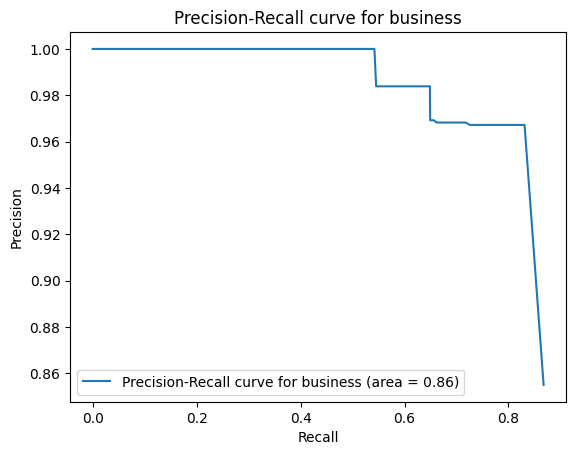
\includegraphics[width=1\linewidth]{images/pr_question_1_part1.png}
    \captionof{figure}{First Part Approach}
    \label{fig:firstpart}
  \end{minipage}%
  \begin{minipage}{.5\textwidth}
    \centering
    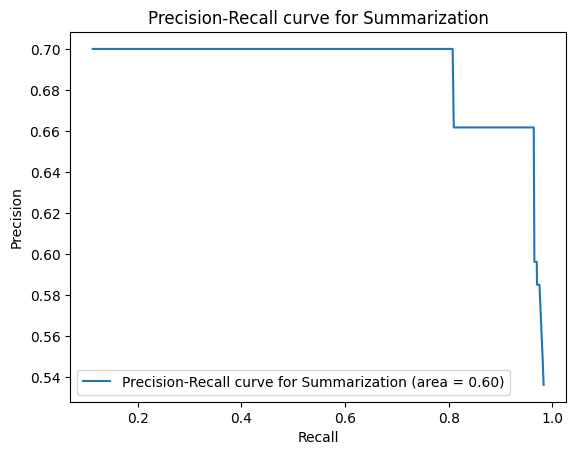
\includegraphics[width=1\linewidth]{images/pr_question_1.png}
    \captionof{figure}{Clustered Approach}
    \label{fig:clustered}
  \end{minipage}
\end{figure}

This result doesn't guarantee that the \textbf{clustering based} approach is
worse than the approach using TFIDF and BM25, because this is based on our
personal implementation of the algorithm. However, it is clear that the
clustering approach is not as effective as the first approach in this case. A
possible way to improve the algorithm could be to consider other sentences
choices rather than focusing on the distance from the centroid of each cluster.

\subsection{Question 2}
\textbf{How sentence representations, clustering choices, and rank criteria impact summarization?}

We benchmarked the performance of the clustering algorithm using a set of
metrics:
\begin{table}[H]
  \centering
  \begin{tabular}{|c|c|c|}
    \hline
    \textbf{Max Clusters} & \textbf{Number of Sentences} & \textbf{Our Metrics} \\
    \hline
    2                     & 3                            &                      \\
    3                     & 5                            &                      \\
    4                     & 7                            & cosine               \\
    6                     & 9                            & euclidean            \\
    8                     & 11                           &                      \\
    10                    & 13                           &                      \\
    \hline
  \end{tabular}
\end{table}

We didn't include any \textbf{different representations} because we only used
the \textbf{TFIDF} representation. The result are indicating a very low
performance of the algorithm using a specific set of metrics.

\begin{table}[H]
  \centering
  \caption{Results of the clustering algorithm using different metrics}
  \label{tab:my-table}
  \begin{adjustbox}{margin={-1cm 0cm 0cm 0cm}}
    \begin{tabular}{|c|c|c|c|c|c|c|c|}
      \hline
      \textbf{\#cluters} & \textbf{\#sentences} & \textbf{metric} & \textbf{avg\_prec} & \textbf{avg\_rec} & \textbf{f1} & \textbf{m\_a\_p} \\ \hline
      2                  & 3                    & cosine          & 0.453504           & 0.449012          & 0.451247    & 0.646069         \\ \hline
      2                  & 3                    & euclidean       & 0.453504           & 0.449012          & 0.451247    & 0.646069         \\ \hline
      2                  & 5                    & cosine          & 0.457060           & 0.633170          & 0.530891    & 0.561392         \\ \hline
      2                  & 5                    & euclidean       & 0.457060           & 0.633170          & 0.530891    & 0.561392         \\ \hline
      2                  & 7                    & cosine          & 0.469898           & 0.768889          & 0.583312    & 0.492352         \\ \hline
      ...                & ...                  & ...             & ...                & ...               & ...         & ...              \\ \hline
      10                 & 9                    & euclidean       & 0.484872           & 0.934921          & 0.638568    & 0.418472         \\ \hline
      10                 & 11                   & cosine          & 0.486431           & 0.941682
                         & 0.641495             & 0.344811                                                                                  \\ \hline
      10                 & 11                   & euclidean       & 0.486431           & 0.941682          & 0.641495    & 0.344811         \\ \hline
      10                 & 13                   & cosine          & 0.486635           & 0.943571          & 0.642110    & 0.336604         \\ \hline
      10                 & 13                   & euclidean       & 0.486635           & 0.943571          & 0.642110    & 0.336604         \\ \hline
    \end{tabular}
  \end{adjustbox}
\end{table}

More insight on this can be found in the \textit{notebook} file.

\subsection{Question 3}
\textbf{ Are anchor sentences (capturing multiple topics) included? And less relevant outlier sen- tences excluded? Justify}

Since our algorithm is based on the \textbf{distance from the centroid} of each
cluster to select the sentences, we are not able to handle the \textbf{anchor
  sentences} and the \textbf{outlier sentences}. We are not able to give a clear
answer to this question, but a possible way to handle this could be to consider
the \textbf{distance from the centroid} and the \textbf{distance from the other
  sentences} inside other clusters. Sentences that are \textbf{more far} from the
centroid of the cluster could be very \textbf{relevant} and could be considered
as \textbf{anchor sentences}, since that sentence could be holding information
between more topics.

\subsection{Question 4}
\textbf{Given a set of documents, plot the distribution of the number of keywords per document. Are keywords generally dissimilar? If not, how would you tackle this challenge?}
For this question we decided to use documents from \textbf{500} to \textbf{700} as range. 
The result shows that the distribution of the number of keywords per
document is not uniform.

\begin{figure}[H]
  \begin{minipage}{.5\textwidth}
    \centering
    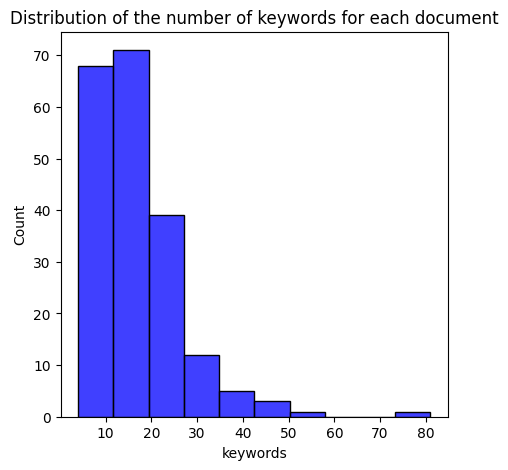
\includegraphics[width=1\linewidth]{images/keyword_distribution.png}
    \captionof{figure}{Distribution of the number of keywords per document}
    \label{fig:question4_1}
  \end{minipage}
  \begin{minipage}{.5\textwidth}
    \centering
    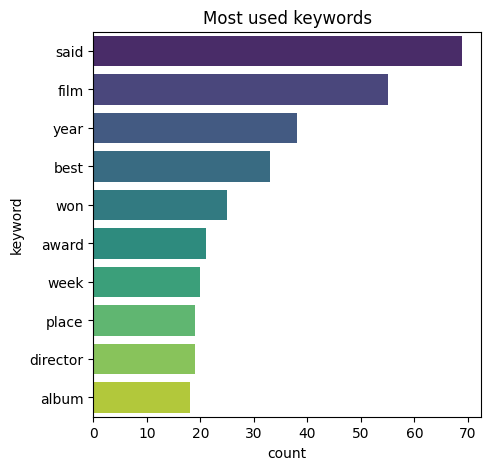
\includegraphics[width=1\linewidth]{images/keyword_distribution_ranks.png}
    \captionof{figure}{Distribution of the number of keywords per document}
    \label{fig:question4_2}
  \end{minipage}
\end{figure}

We can note that the \textbf{keywords} is not \textbf{uniformly distributed} in 

\section*{Part B: Supervised IR}
\subsection{Question 1}
\textbf{ Does the incorporation of relevance feedback from ideal extracts significantly impact the performance of the IR system? Hypothesize why is that so.}

\subsection{Question 2}
\textbf{ Are the learned models able to generalize from one category to another? Justify.}
\subsection{Question 3}

\textbf{Which features appear to be more relevant to the target summarization task? Do sentence- location features aid summarization?}

\subsection{Question 4}
\textbf{In alternative to the given reference extracts, consider the presence of manual abstractive summaries, can supervised IR be used to explore such feedback? Justify}





\end{document}
